\documentclass{article}%[12pt, a4paper]{article}

\usepackage{ucs}
\usepackage[russian]{babel}
\usepackage{cmap}
\usepackage[utf8x]{inputenc}
\usepackage{amsthm}
\usepackage{amsmath}
\usepackage{amssymb}
\usepackage{graphicx}
\usepackage{float}
\usepackage{clrscode}
\usepackage{tocloft}
\usepackage[usenames]{color}
\usepackage[margin=20mm]{geometry}
\usepackage{sidecap}
\usepackage{url}
\usepackage{hyperref}

\frenchspacing



\begin{document}

\thispagestyle{empty}

\begin{frame}
  \maketitle
\end{frame}

\setcounter{page}{1}

\begin{frame}
  \frametitle{Содержание} 
  Введение \\[0.3cm]
  \tableofcontents
  Заключение \\[0.3cm]
  Использованные источники
\end{frame}

\section*{Введение}
\subsection{Определение}

\begin{frame}
  \frametitle{Введение}
  \framesubtitle{Определение(1)}

  \begin{columns}
    \begin{column}{0.5\textwidth}
       \begin{itemize}
         \item Химическая информатика
         \item Хемоинформатика
       \end{itemize}
    \end{column}
    \begin{column}{0.5\textwidth}
       \begin{itemize}
         \item Chemical informatics
         \item Chem-, chemo- informatics
       \end{itemize}
    \end{column}
  \end{columns}

  \begin{defn}[Ф.К.Браун, 1998]
     Хемоинформатика означает совместное использование информационных ресурсов для преобразования данных
     в информацию и информации в знания для быстрейшего принятия наилучших решений при поиске соединений
     в разработке лекарств и их оптимизации 
  \end{defn}

\end{frame}

\begin{frame}
  \frametitle{Введение}
  \framesubtitle{Определение(2)}

  \begin{defn}[Г.Пэриз, <<Новартис>>]
    Хемоинформатика это научная дисциплина, охватывающая дизайн, создание, организацию, управление, поиск, 
    анализ, распространение, визуализацию и использование химической информации
  \end{defn}

  \begin{defn}[И.Гастайгер]
    Хемоинформатика это применение методов информатики для решения химических проблем
  \end{defn}

  \begin{defn}[Р.Грин]
    Хемоинформатика - новое название старых проблем
  \end{defn}
 
\end{frame}

\subsection{Хемоинформатика и другие науки}

\begin{frame}
  \frametitle{Введение}
  \framesubtitle{Хемоинформатика и другие науки(1)}
  \begin{columns}
    \begin{column}{0.5\textwidth}
      \begin{itemize}
   \item  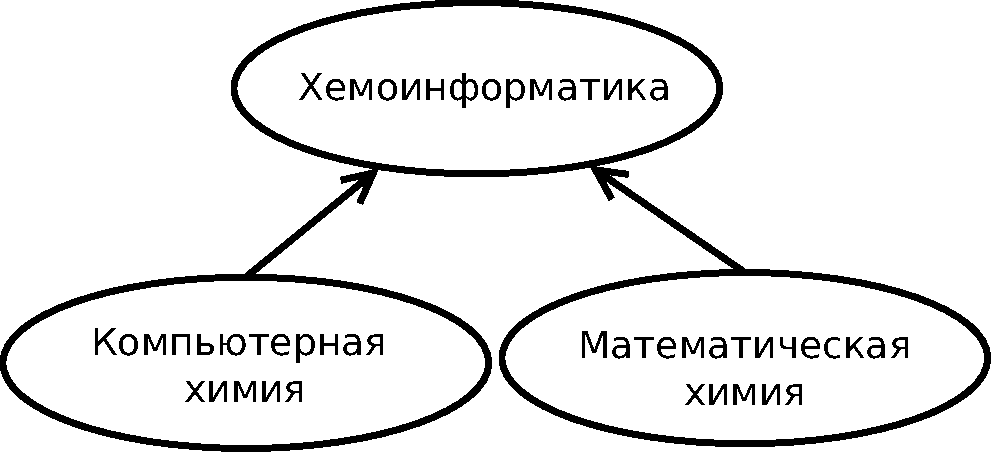
\includegraphics[scale=0.32]{images/Diagram1.pdf}
   \item  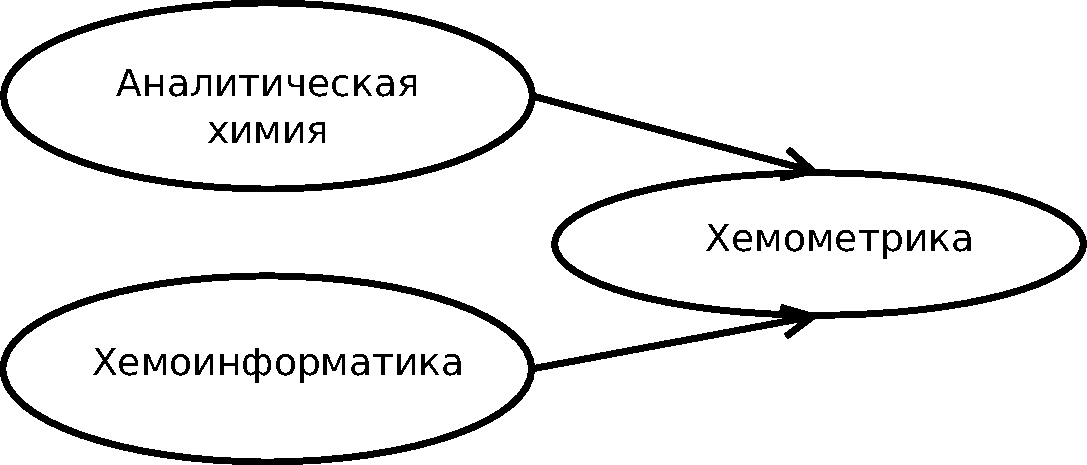
\includegraphics[scale=0.3]{images/Diagram3.pdf}
      \end{itemize}
    \end{column}
    \begin{column}{0.5\textwidth}      
      \begin{itemize}
      \item 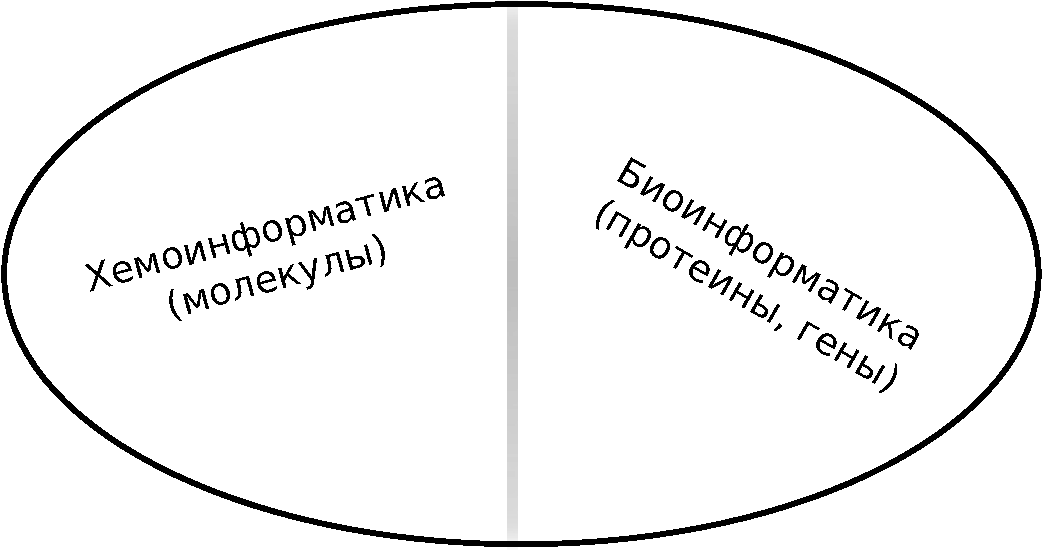
\includegraphics[scale=0.3]{images/Diagram2.pdf}
      \item 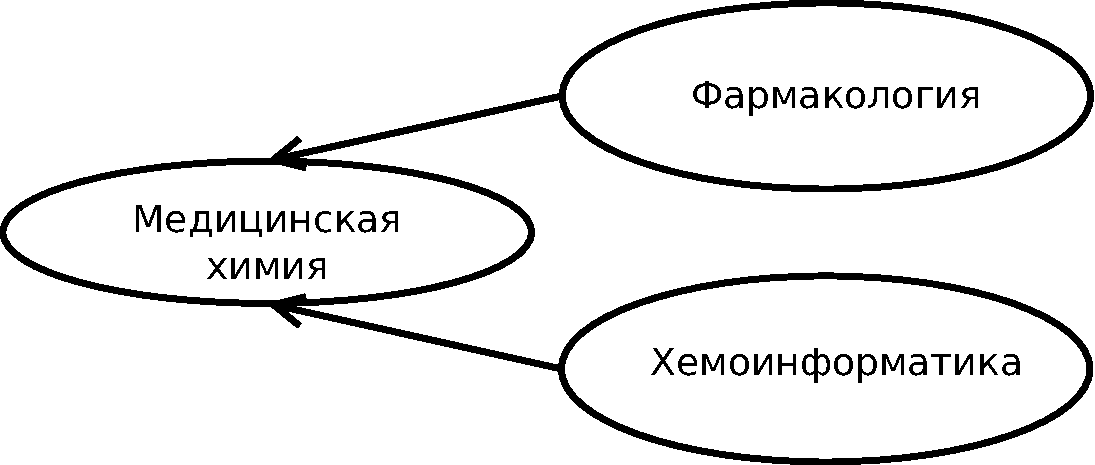
\includegraphics[scale=0.29]{images/Diagram4.pdf}
      \end{itemize}
    \end{column}
  \end{columns}
\end{frame}

\begin{frame}
  \frametitle{Введение}
  \framesubtitle{Хемоинформатика и другие науки(2)}

  \begin{center}
    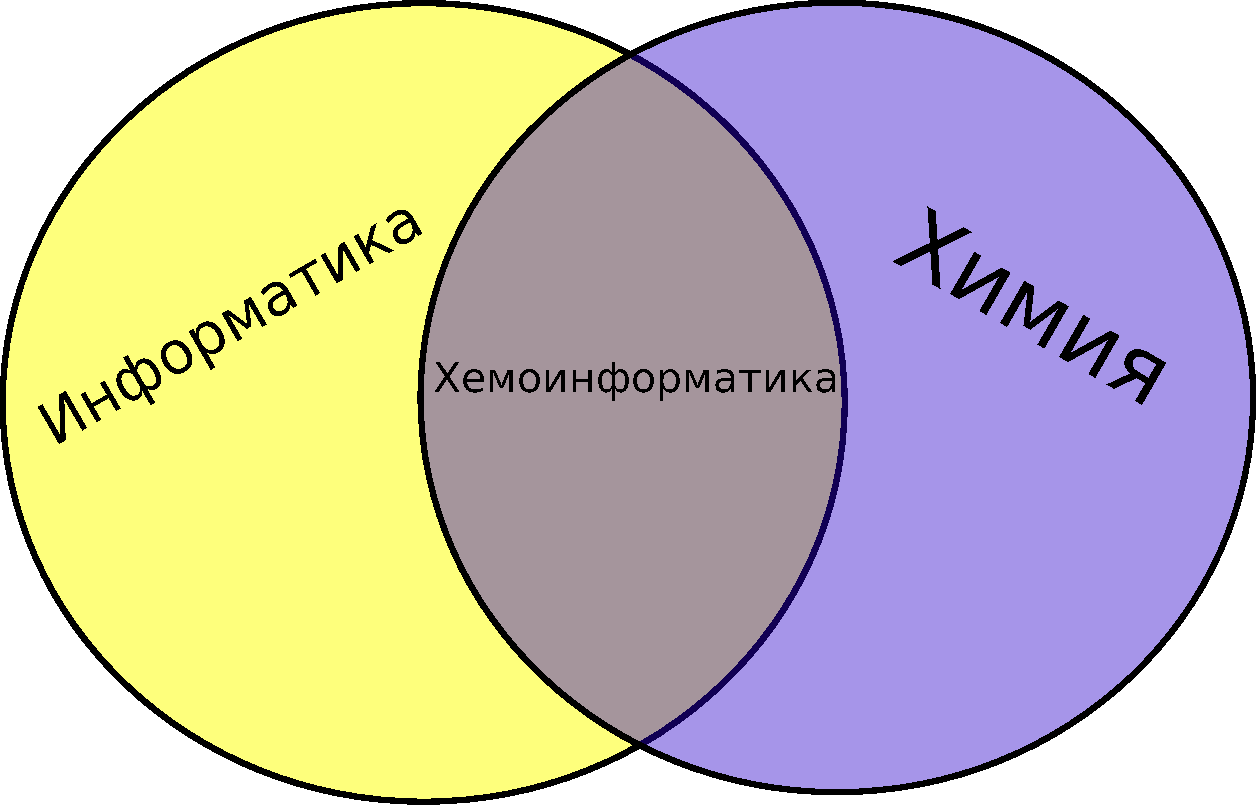
\includegraphics[scale=0.3]{images/Diagram5.pdf}
  \end{center}

  Основные используемые инструменты информатики и математики:
  \begin{columns}
    \begin{column}{0.5\textwidth}
  \begin{itemize}
    \item Базы данных
    \item Интеллектуальный анализ данных
    \item Математическая статистика
   \end{itemize}
\end{column}
\begin{column}{0.5\textwidth}
  \begin{itemize}
   \item Машинное обучение
    \item Теория графов
    \item Компьютерная графика
      \end{itemize}

\end{column}
\end{columns}
\end{frame}

\section{Фундаментальные вопросы}
\begin{frame}
   \frametitle{Фундаментальные вопросы}
   \begin{columns}
      \begin{column}{0.6\textwidth}
      \begin{enumerate}
         \item Какое {\color{red}химическое соединение} обладает интересующим свойством? \\
            \emph{Свойство} $ \rightarrow $ \emph{Структура}
         \item Как получить такое {\color{red}химическое соединение}? \\
            \emph{Исходные вещества} $ \rightarrow $ \emph{Соединение}
         \item Какое {\color{red}химическое соединение} получится в результате реакции? \\
            \emph{Реакция} $ \rightarrow $ \emph{Продукт}
      \end{enumerate}
      \end{column}
      \begin{column}{0.4\textwidth}
         
\includegraphics[scale=0.65]{images/question-marks2.png}
      \end{column}
   \end{columns}
\end{frame}

\begin{frame}
  \frametitle{Причины появления хемоинформатики}
  \begin{columns}
    \begin{column}{0.5\textwidth}
  \begin{itemize}
    \item Огромное количество информации: миллионы соединений, миллионы публикаций
    \item Сложные химико-биологические связи
      \begin{itemize}
        \item Потребность в математических расчетах
        \item Потребность в визуализации
      \end{itemize}
    \item Низкая результативность экспериментов
    \item Дороговизна натурных экспериментов
    \item Вечный поиск новых лекарств
  \end{itemize}
   \end{column}
   \begin{column}{0.5\textwidth}
     \centering 
\includegraphics[scale=0.2]{images/sad.png} \\ 
     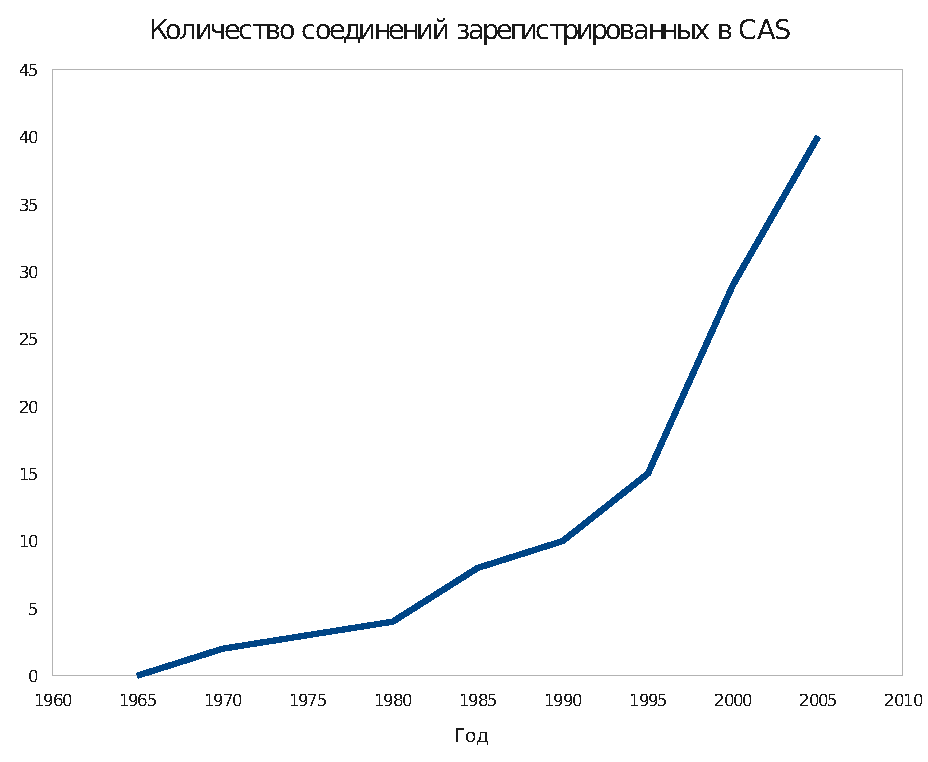
\includegraphics[scale=0.35]{images/graph.pdf}
   \end{column}
 \end{columns}

 \footnotetext[1]{CAS: Chemical Abstracts Service, химическая реферативная служба}

\end{frame}

\section{История}

\begin{frame}
   \frametitle{История}
   \framesubtitle{Первые <<хемоинформатики>>}
   \begin{center}
   \begin{tabular}{c c}
     Дмитрий Иванович Менделеев & Фридрих Август Кекуле \\
     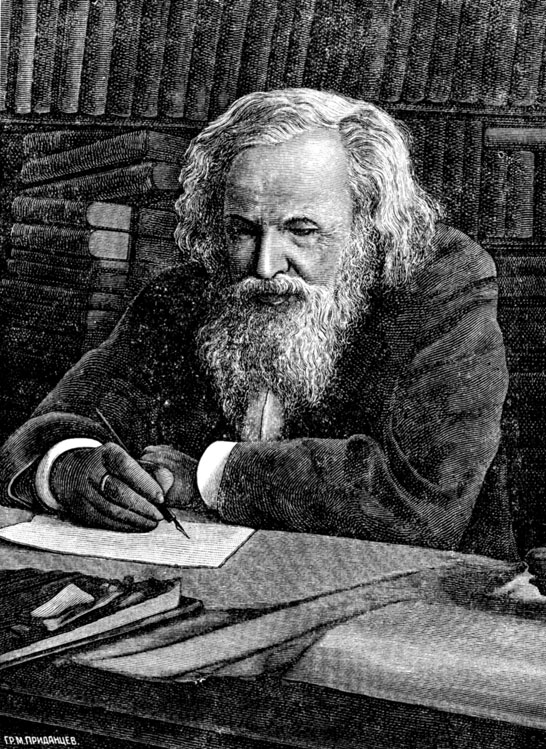
\includegraphics[scale=0.25]{images/mendeleev.png} & 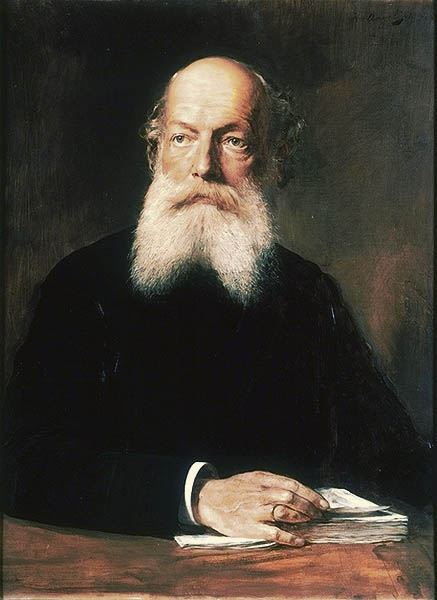
\includegraphics[scale=0.31]{images/kekule.png} \\
   \end{tabular}
 \end{center}
\end{frame}

\begin{frame}
  \frametitle{История}
  \framesubtitle{Вехи зарождения}
  \begin{itemize}
    \item Базы данных
      \begin{itemize}
        \item 1957 год. Вашингтон, Национальное Бюро Стандартов
        \item 1960 год. Начало финансирования Химической Реферативной Службы для составления баз данных и разработки методов поиска          
      \end{itemize}
    \item Визуализация
      \begin{itemize}
        \item Конец шестидесятых. Принстон и Сан-Франциско
      \end{itemize}
        \item Разработка синтеза
          \begin{itemize}
            \item 1969 год. Гарвард
          \end{itemize}
        \item Структурное разъяснение \emph{(elucidation)} и генерация химических соединений
          \begin{itemize}
            \item 1964 год. Стэнфорд, проект \begin{tt}DENDRAL\end{tt}
            \item 1970 год. Университет Аризоны
          \end{itemize}
  \end{itemize}
\end{frame}

\section{Представление химической информации}
\subsection{Внутреннее}
\begin{frame}
  \frametitle{Представление химической информации}
  \framesubtitle{Внутреннее: модель молекулярного графа(1)}
   \begin{columns}
    \begin{column}{0.6\textwidth}
      \begin{tabular}{|c|c|}
      \hline Химия & Теория графов \\ \hline
      {\color{magenta}Молекула} & {\color{orange}Связный компонент} \\ \hline
      {\color{magenta}Атом} & {\color{orange}Вершина} \\ \hline
      {\color{magenta}Связь} & {\color{orange}Ребро} \\ \hline
      {\color{magenta}Название атома} & {\color{orange}Метка вершины} \\ \hline
      {\color{magenta}Порядок связи} & {\color{orange}Метка ребра} \\ \hline
      {\color{magenta}Валентность атома} & {\color{orange}Степень вершины} \\ \hline
      \end{tabular} \\
    \end{column}
    \begin{column}{0.2\textwidth}    
      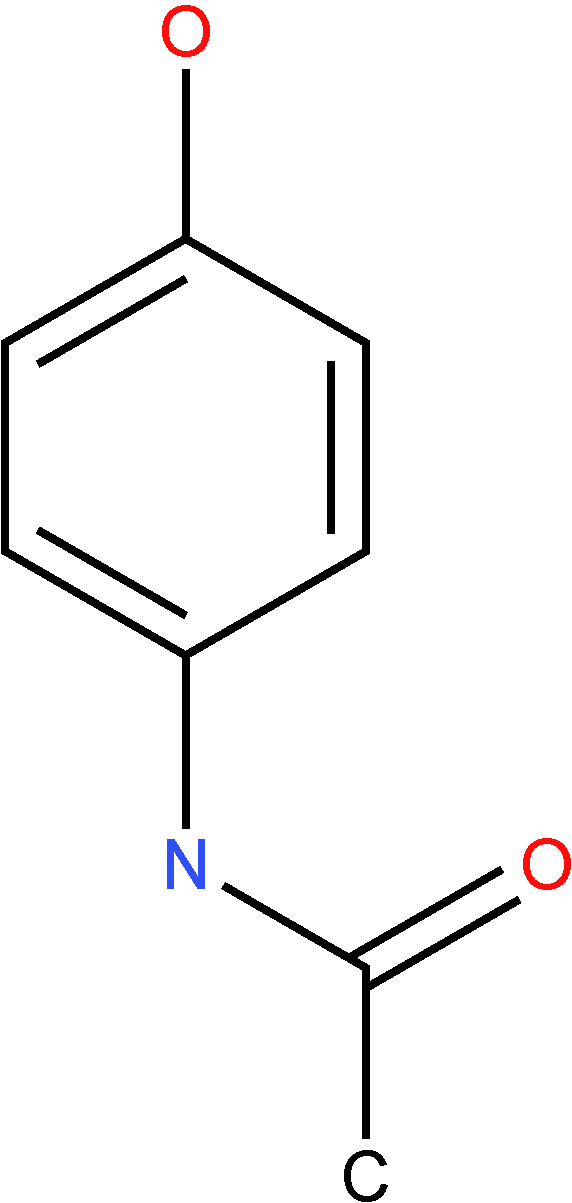
\includegraphics[scale=0.3]{images/Diagram6.pdf}      
    \end{column}
   \end{columns}
   Изоморфизм структурной формулы молекулы и молекулярного графа
\end{frame}

\begin{frame}
  \frametitle{Представление химической информации}
  \framesubtitle{Внутреннее: модель молекулярного графа(2)}
  \begin{center}
  \begin{tabular}{|m{5cm}|m{5cm}|}
      \hline Химия & Теория графов \\ \hline
      {\color{magenta}Свойство молекулы,} & {\color{orange}Инвариант графа} \\ 
      {\color{magenta}дескриптор молекулы} & \\ \hline
      {\color{magenta}Одинаковые молекулы} & {\color{orange}Изоморфные графы} \\ \hline
      {\color{magenta}Наличие определенного} & {\color{orange}Изоморфизм графа подграфу}  \\
      {\color{magenta}фрагмента в молекуле} & \\ \hline
      {\color{magenta}Поиск подструктуры} & {\color{orange}Поиск изоморфного} \\ & {\color{orange}подграфа} \\ \hline
      {\color{magenta}Пересечение молекул} & {\color{orange}Максимальный общий} \\ & {\color{orange}подграф} \\ \hline
      {\color{magenta}Порядок связи} & {\color{orange}Метка ребра} \\ \hline
      {\color{magenta}Топологическая группа} & {\color{orange}Группа автоморфизмов} \\ 
      {\color{magenta}симметрий} & {\color{orange}графа} \\ \hline
  \end{tabular} 
\end{center}
\end{frame}

\subsection{Внешнее}
\begin{frame}
  \frametitle{Представление химической информации}
  \framesubtitle{Внешнее: химические форматы файлов(1)}
  \begin{columns}
\begin{column}{0.7\textwidth}
  \begin{itemize}
    \item Строковое представление, \begin{tt}SMILES\end{tt}\footnotemark 
      \begin{itemize}
        \item Метан $ CH_4 \overset{SMILES}{\rightarrow} C $
        \item Этанол $ C_2H_6O \overset{SMILES}{\rightarrow} CCO $
        \item Бензол $ C_6H_6 \overset{SMILES}{\rightarrow} C1=CC=CC=C1 $
      \end{itemize}
    \item Строковое представление, \begin{tt}InChi\end{tt}\footnotemark
        \begin{itemize}
          \item Этанол \\ $ C_2H_6O \overset{InChi}{\rightarrow} InChi=1/C2H6O/c1-2-3/h3H,2H2,1H3 $
        \end{itemize}
      \item Представление с помощью языка разметки, \begin{tt}CML\end{tt}\footnotemark
            \end{itemize}
\end{column}
    \begin{column}{0.5\textwidth}
  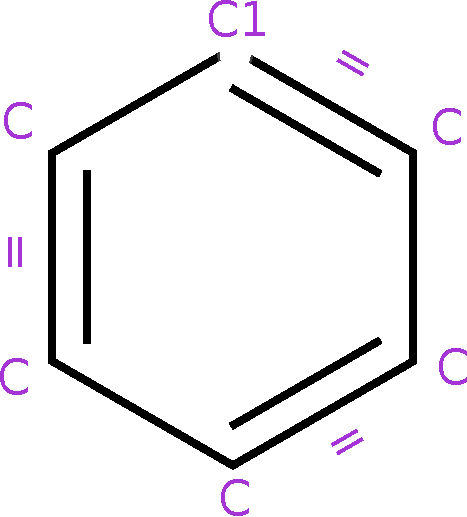
\includegraphics[scale=0.4]{images/benzene.pdf}
\end{column}

\end{columns}
   \footnotetext[2]{Simplified Molecular Input Line Entry Specification} 
   \footnotetext[3]{IUPAC International Chemical Identifier}
   \footnotetext[4]{Chemical Markup Language}
\end{frame}

\begin{frame}
  \frametitle{Представление химической информации}
  \framesubtitle{Внешнее: химические форматы файлов(2)}
  \begin{itemize}
    \item Формат \begin{tt}XYZ\end{tt} $=$ метки атомов $+$ их координаты. Отражает геометрию молекулы.
    \item Табличное представление, \begin{tt}MDL\footnotemark Molfile\end{tt} \footnotetext[5]{Molecular Design Limited, Inc.}
    \item Табличное представление, \begin{tt}SDF\end{tt}\footnotemark \footnotetext[6]{Structure-Data File}
  \end{itemize}
  \begin{center}
   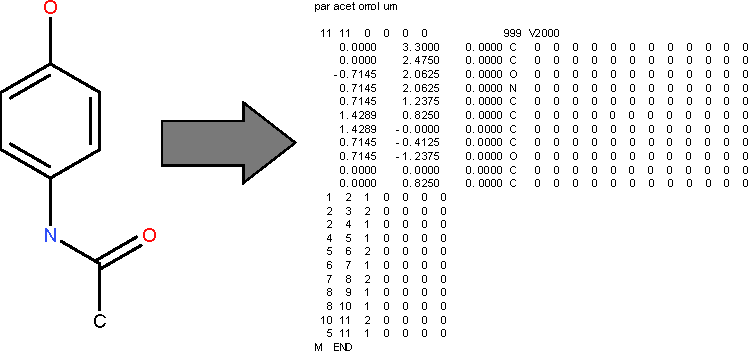
\includegraphics[scale=0.70]{images/parac.pdf}
  \end{center}
\end{frame}

\section{Программные решения}
\begin{frame}
  \frametitle{Программные решения}
  \framesubtitle{Базы данных: химические соединения}
  Химический картридж
  \begin{itemize}
    \item Поисковый движок для базы данных химических соединений 
    \item Программа, расширяющая функциональность СУБД и позволяющая работать с ней в терминах предметной области
  \end{itemize}
  \begin{columns}
    \begin{column}{0.5\textwidth}
  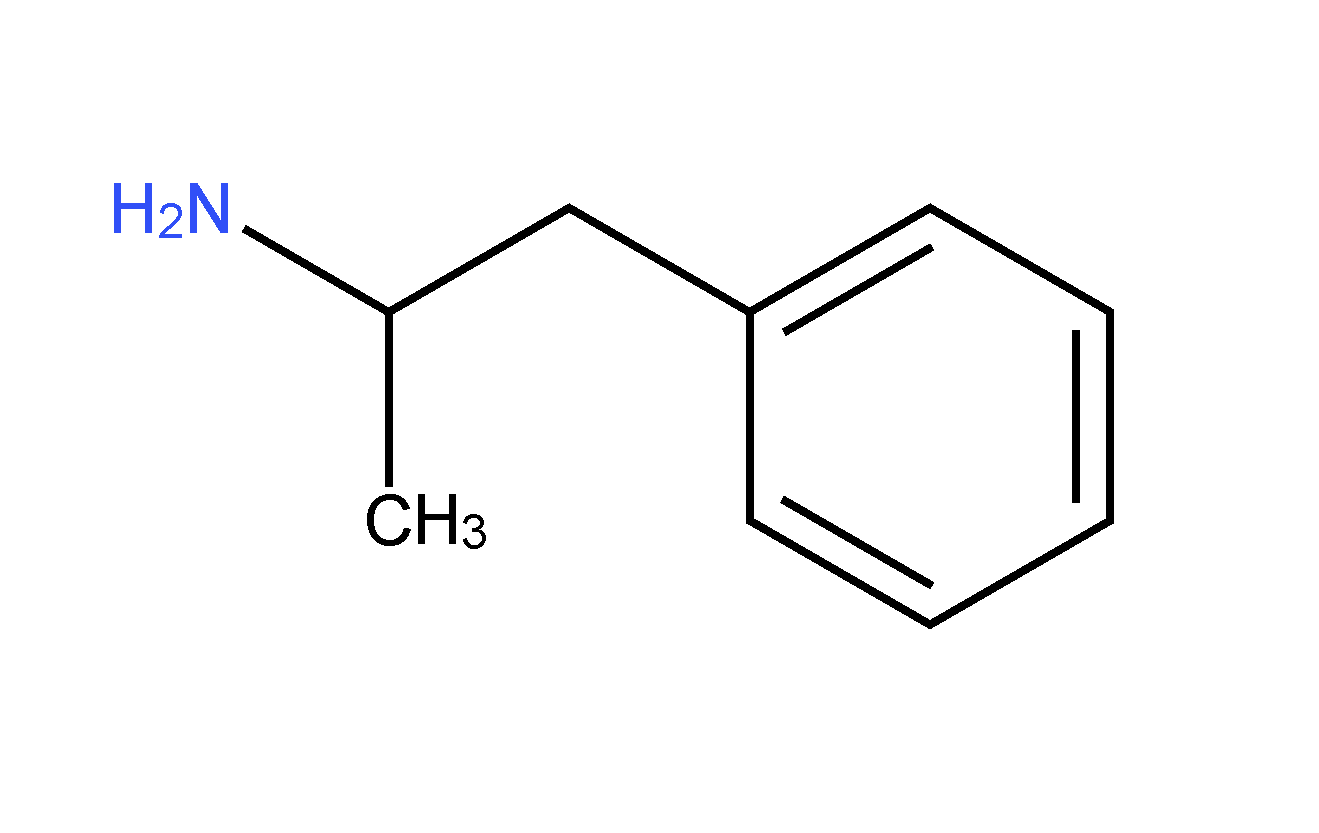
\includegraphics[scale=0.2]{images/amphetamine.pdf} \\
  Возникают сложные задачи теории графов
\end{column}
\begin{column}{0.5\textwidth}
 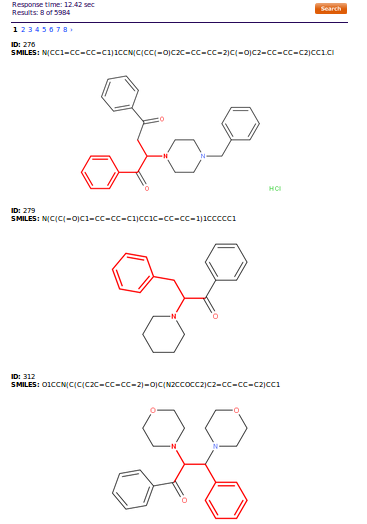
\includegraphics[scale=0.38]{images/substructure_search.png}
\end{column}
\end{columns}
  \end{frame}

\begin{frame}
  \frametitle{Программные решения}
  \framesubtitle{Поиск количественных соотношений структура-свойство (QSAR\footnotemark)}

  \begin{center}Отображение химического пространства на пространство дескрипторов\end{center}
    \begin{columns}
      \begin{column}{0.5\textwidth}
        \begin{itemize}
        \item Фрагментные бинарные и целочисленные дескрипторы или структурные ключи
        \item Физико-химические дескрипторы
        \item Квантово-химические дескрипторы
        \item Топологические индексы
        \item Дескрипторы молекулярных полей
        \end{itemize}
      \end{column}
      \begin{column}{0.5\textwidth}
        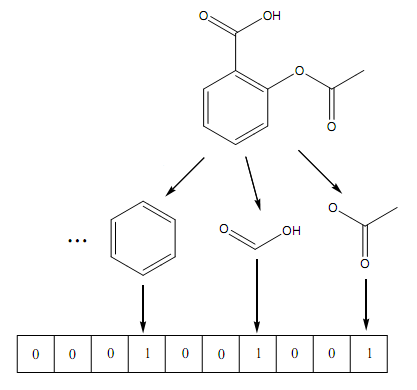
\includegraphics[scale=0.5]{images/screens.png}
      \end{column}
    \end{columns}
  \footnotetext[7]{QSAR: Quantative structure-activity relationship}
\end{frame}

\begin{frame}
  \frametitle{Программные решения}
  \framesubtitle{Молекулярные дескрипторы(1)}
  \begin{itemize}
    \item Дескрипторный подход - другое представление химической информации, неграфовое. 
    \item При прогнозировании свойств
  различают две задачи:
  \begin{itemize}
    \item Классификационная - качественный уровень
    \item Регрессионная - числовые значения
  \end{itemize}
  \end{itemize}
  Применяются методы математической статистики и машинного обучения 
\end{frame}

\begin{frame}
   \frametitle{Программные решения}
   \framesubtitle{Молекулярные дескрипторы(2)}
   Дескрипторы применяются не только для прогнозирования свойств соединений   
   \begin{columns}
     \begin{column}{0.4\textwidth}
       \begin{itemize}
         \item Ускорение подструктурного поиска
         \item Задача молекулярного подобия
         \item Нахождение одинаковых соединений
       \end{itemize}
     \end{column}
     \begin{column}{0.6\textwidth}
   \begin{center}
    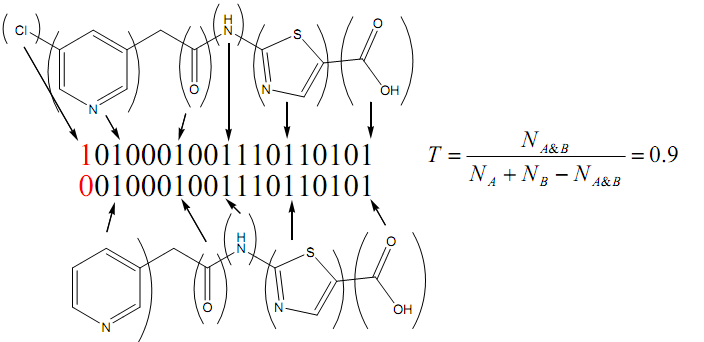
\includegraphics[scale=0.4]{images/similarity.png}
   \end{center}
   \end{column}
   \end{columns}
\end{frame}

\begin{frame}
  \frametitle{Программные решения}
  \framesubtitle{Базы данных: публикации}
    Найденные в базе данных молекулы не очень интересны сами по себе \\
    Интересен контекст:
    \begin{center}
    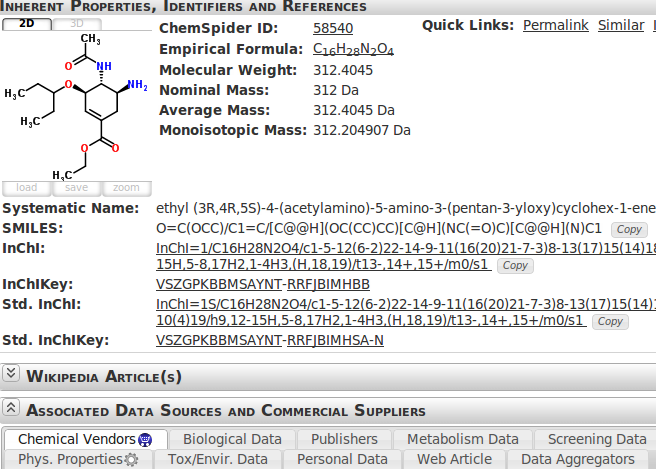
\includegraphics[scale=0.42]{images/chemspider.png}
    \end{center}
    \begin{center}Возникают задачи интеллектуального анализа данных \end{center}
\end{frame}

\begin{frame}
  \frametitle{Программные решения}
  \framesubtitle{Редакторы молекул}

  \begin{center}
    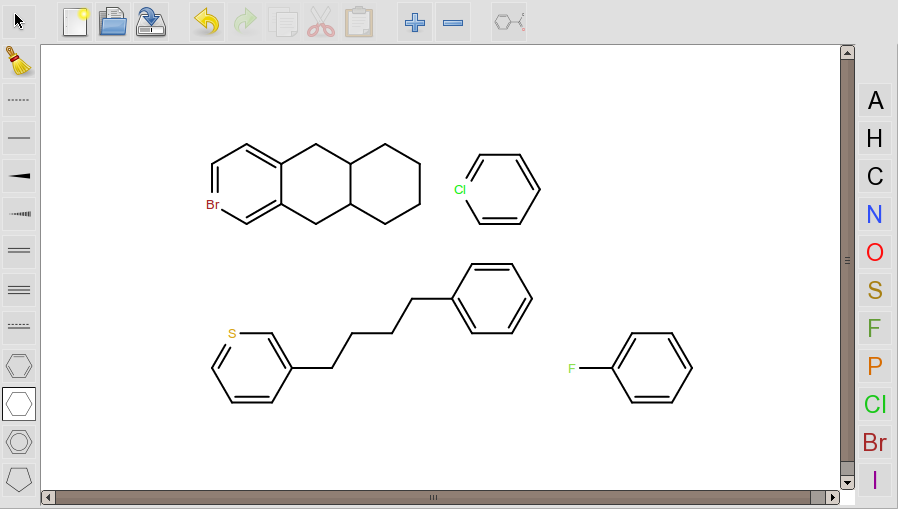
\includegraphics[scale=0.37]{images/sketcher.png}
  \end{center}
  \begin{itemize}
    \item Возникают задачи укладки графа на плоскости, создание общего стандарта отрисовки, эстетики рисунка 
  \end{itemize}

\end{frame}

\begin{frame}
  \frametitle{Программные решения}
  \framesubtitle{Докинг или молекулярная стыковка}
  \begin{columns}
    \begin{column}{0.5\textwidth}
      \begin{itemize}
        \item Метод, позволяющий предсказать наиболее выгодную для создания устойчивого комплекса ориентацию и положение
          одной молекулы относительно другой
      \end{itemize}
    \end{column}
    \begin{column}{0.5\textwidth}
  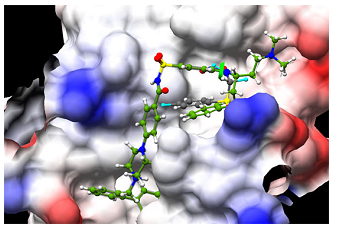
\includegraphics[height=1.3in]{images/docking.png}
\end{column}
\end{columns}
   \begin{center} Возникают задачи оптимизации \end{center}
\end{frame}

\section{Актуальные проблемы}
\begin{frame}
  \frametitle{Актуальные проблемы}
  \begin{columns}
    \begin{column}{0.7\textwidth}
  \begin{itemize}
    \item \emph{in silico} contra \emph{in vivo} et \emph{in vitro}
    \item Некачественное программное обеспечение для исследователей
      \begin{itemize}
        \item Пользовательские интерфейсы
        \item Производительность
      \end{itemize}
    \item Разобщенность обладателей баз данных, отсутствие стандартов 
  \end{itemize}
   \end{column}
   \begin{column}{0.2\textwidth}
     
\includegraphics[scale=0.5]{images/mouse.pdf}
   \end{column}
   \end{columns}
\end{frame}

\section*{Заключение}
\begin{frame}
  \frametitle{Заключение}
  \begin{itemize}
    \item Хемоинформатика - сравнительно молодая область
    \item Роль информатики в химии и фармакологии высока уже сейчас 
      \begin{itemize}
        \item Дороговизна натурных экспериментов
        \item Очень долгий срок разработки лекарства
      \end{itemize}
    \item Химия нуждается в информатике и математике
      \begin{itemize}
    \item Создаются университетские специальности по хемо- и биоинформатике
    \item Проводятся конференции
  \end{itemize}

  \end{itemize}
\end{frame}

\section*{Использованные источники}

\begin{frame}
  \frametitle{Использованные источники}
  \framesubtitle{Книги}
  \begin{enumerate}
    \item J.Gasteiger, T.Angel \emph{Chemoinformatics: A Textbook}, 2003     
    \item F.K.Brown \emph{Chemoinformatics: What is it and How does it Impact Drug Discovery}, 1998
    \item B.A.Bunin, B.Siesel, G.A.Morales, J.Bajorath \emph{Chemoinformatics: Theory, Practice, \& Products}, 2007
    \item A.R.Leach, V.J.Gillet \emph{An introduction to chemoinformatics}, 2007
  \end{enumerate}
\end{frame}

\begin{frame}
  \frametitle{Использованные источники}
  \framesubtitle{Журналы, презентации, интернет}
  \begin{enumerate}
    \item Дмитрий Павлов, \emph{Навигация в мире органических соединений}, Компьютерные инструменты в образовании, 2010, №3 
    \item Сергей Кокорин, \emph{Заметки о Cheminfo'S. Strasbourg Summer School on Chemoinformatics.} 
    \item Материалы AACIMP-2008, курс ``Хемоинформатика'' \\ 
	       \url{http://summerschool.ssa.org.ua/}
    \item Noel O'Boyle, \emph{http://baoilleach.blogspot.com/}
    \item Википедия (русская, английская)
   \end{enumerate}

\end{frame}

\begin{frame}
   \begin{center}
   \LARGEСпасибо за внимание!
   \end{center}
\end{frame}

\end{document}

